\chapter{Implementation}
\label{cha:implementation}
In this chapter, we describe how we implemented the simulation. Section~\ref{sec:components} presents the various components we developed by describing what their task is, what we noticed during the implementation and why we implemented them this way. In section~\ref{sec:agent_improvements}, we present the improvements of the multi-agent system we implemented during this thesis.

\section{Components}
\label{sec:components}
As shown in Figure~\ref{fig:fawkes_gazebo}, we need to implement three basic parts to be able to run the robot software in the simulation. On the one hand, we need to implement the simulation environment with the objects appearing in the LLSF and the Gazebo plugins to define the behavior of these objects, to send sensor data to Fawkes and to execute received actuator commands. On the other hand, we need to implement the simulation plugins in Fawkes which communicate with the simulation and provide all required Fawkes-interfaces for the robot control plugins.

\subsection{Gazebo Models}
\begin{figure}
\centering
\begin{subfigure}[b]{0.48\textwidth}
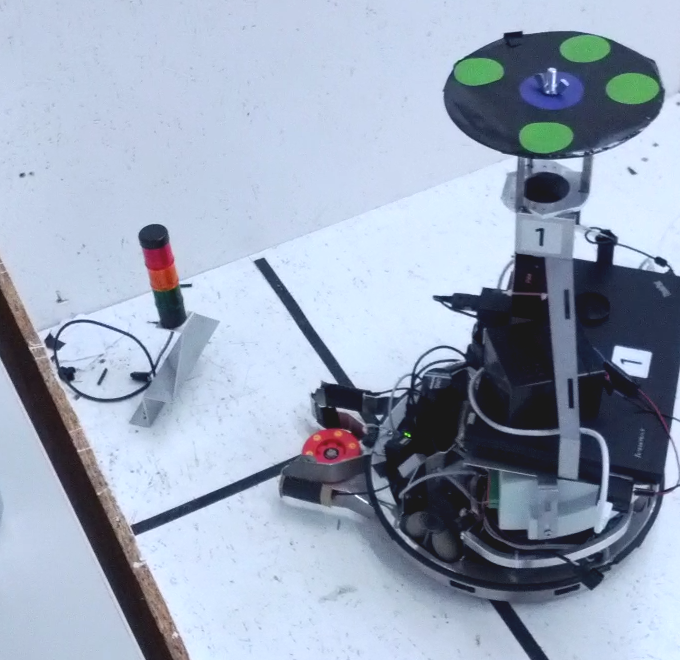
\includegraphics[width=\textwidth]{pics/llsf_real}
\caption{A Robotino delivers a puck to a recycling machine.}
\label{fig:comparison_real}
\end{subfigure}
\begin{subfigure}[b]{0.48\textwidth}
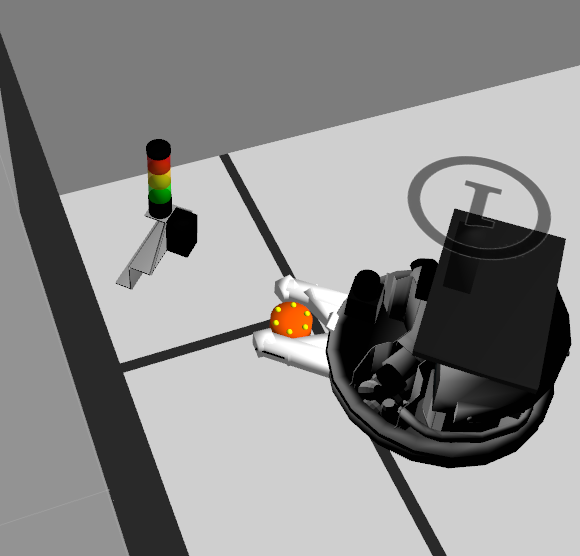
\includegraphics[width=\textwidth]{pics/llsf_sim}
\caption{The same situation in the Gazebo~simulation}
\label{fig:comparison_sim}
\end{subfigure}
\caption{Comparison of the real scene and the simulated scene in Gazebo}
\label{fig:comparison}
\end{figure}

In order to simulate the LLSF environment, we need to model all objects appearing in this domain\footnote{The models developed in this thesis are available at \url{https://github.com/zwilling/llsf-models.git}.}. Here, we present our simulation models and why we modeled them this way. Figure~\ref{fig:comparison} shows a comparison between a real LLSF scene and the same scene in the simulation. In this comparison, the most important objects of the simulation can be seen. In the following, we describe each model in detail:\\
\textbf{LLSF Field:} The model of the LLSF field has a rather simple structure. It consists of a ground plane and four side walls. For the visual appearance and possible future changes, the field has a visual representation with lines and colored areas just as the real field. The machines are not implemented as a component of the field. Instead they are separate models attached to the field in the description of the simulation world.\\
\textbf{Machine:} The model of the machines matche their real counterpart structurally. Though, it is challenging to represent the lamps consisting of colored and transparent plastic with an LED inside. We decided to use simple colored cylinders in the simulation. If the lamp is turned off, we use a dark and slightly transparent color and, if the light is turned on, we use a bright color. This looks reasonable in the simulation and the images from the simulation are sufficient for our vision plugin which determines light states of the machines. The vision plugin measures the brightness at the position where it expects the machine-lamp to be and it even was not necessary to change brightness thresholds. In Figure~\ref{fig:comparison_real}, the black RFID box at the front of the machine is missing because we do not have RFID readers.\\
\textbf{Puck:} The visual appearance of the puck model can be seen in Figure~\ref{fig:comparison_sim}. Physically, it is represented by a single cylinder. The difficult part was to find good friction parameters for the surface of the cylinder. On the one hand, it should easily slide across the floor, on the other hand, it should stay inside the puck holder of the Robotino when the Robotino turns. If the friction parameters are too small, the puck moves out of the puck holder during turning due to the centrifugal force.\\
\textbf{Robotino:} The model of the Robotino is the most complex model because it holds different sensors, the casing and the puck holder. It is also the most important model because it represents the robot we want to simulate. The major visual difference between real world and simulation is caused by the missing framework on top of the Robotino and the visual appearance of the puck holder. Both are not important because we do not detect other Robotinos with a camera and the puck detection is currently realized on a higher abstraction level. We detect other Robotinos with the laser sensor. Therefore and because of the manipulation with the puck holder, the physical representation is more important. The physical model of the Robotino is composed of the puck holder and two cylinders, one on the ground to represent the basic circle of the Robotino and one at laser and machine height. The cylinder at laser height is smaller and shifted backwards so it does not block the laser sensor and matches better to the real shape. The real puck holder has a similar shape as in the simulation. We needed to assign higher friction parameters to the inside of the puck holder than to the outside because in reality the puck slides into the puck holder if the front side of the puck holder and stays in the puck holder while turning. Because we were not able to simulate this with a single set of friction parameters, we modeled an additional geometry for the inside of the puck holder with higher friction parameters. Originally, we intended to add wheels to the physical design for the final version of the Robotino. However, the omni-directional wheels caused an abnormal physical behavior in the simulation. The wheels irregularly bounced on the ground because of gravity and collision. Because we could not solve this problem in an arguable time and there is no important advantage, we decided to keep the simple model without wheels. We only loose the possibility to physically simulate odometry with a realistic error. Therefore, we introduced an artificial odometry error in the Gazebo plugin for the Robotino.\\
\textbf{Simulation World:} The world file simply combines the developed models to an LLSF environment. Our world consists of the LLSF field, 16 machines with configurable orientation, 20 pucks and three Robotinos. This is the same setup as in real LLSF games.\\


\subsection{Gazebo Plugins}
In order to control the simulation environment and the models created before, we need Gazebo plugins. Each plugin belongs to an object in the simulation, such as a robot, a sensor or the simulation world. We developed two main plugins, one for a Robotino and one for the simulation world. Both plugins are composed of smaller reusable modules, which can easily and dynamically be turned on and off.

\textbf{World Plugin}
Our Gazebo plugin for the simulation world is called \texttt{llsf\_world}. It manages the LLSF field, collects simulation data which is needed by several plugin instances and sends general simulation information to Fawkes. An important component of \texttt{llsf\_world} is the simulation data table. It contains general data about the simulation and can be used by all plugins. In our case, the table contains machine locations, machine light-signals and puck locations. This simple data table allows decoupling information gathering modules, storage and modules which use this information. This is useful to make the simulation flexible and expandable for future changes. We implemented a module which receives messages from the Refbox about puck states and light states of the machines and writes the information into the data table. Another module uses this data in the data table to apply the light-signals to the visual representation of the machines. Furthermore, there is one plugin, which writes the position of pucks into the data table. The RFID readers are simulated by another module which uses the puck and machine positions. The results are stored in the data table and then sent to the Refbox. We also implemented a module to remove delivered pucks from the field. In reality, the human referee does this task. There is also a module which sends the simulation time to Fawkes for synchronization.

\textbf{Robotino Plugin}
The plugin for the Robotino robot mainly consists of sensor and actuator modules. We have implemented two actuator modules. One simulates the motor. It receives motor commands from Fawkes and applies the motion to the Robotino model. Because setting the velocity in Gazebo only means to apply a corresponding impulse to the model, friction of the model with the ground leads to a resulting velocity which is smaller than the original intended velocity. Therefore, we increase the velocity set to the model so that the resulting velocity is similar to the intended one. The other actuator module operates on a higher abstraction level. It keeps pucks inside the puck holder while the Robotino is turning. This module is optional but useful because it is difficult to simulate the puck in the holder physically correct. The modules we implemented for the sensors can also be separated into low-level and high-level abstraction. On the low abstraction level, we developed modules which use a gyroscope, a laser range finder, a webcam, an infrared distance sensor to detect pucks in the puck holder and digital optical sensors placed at the sides of the puck holder. Most of these modules use sensors defined in the Robotino model. On the high abstraction level, we developed modules for ground truth localization, machine light-signal detection and puck detection. The ground truth localization can be used in Fawkes in exchange of the Adaptive Monte Carlo Localization (AMCL)~\cite{amcl} results we use usually and as a basis to simulate motor odometry. The machine light-signal and puck detection both use the simulation data table so that the multiple Robotino plugin instances do not have gather the information separately.


\subsection{Fawkes Plugins}
The Fawkes plugins developed in this thesis provide access to the simulation in Fawkes. In order to identify plugins for the Gazebo simulation quickly, we named them with the prefix \texttt{gazsim}. We divided the plugins into two groups. The first group of plugins generally covers the access to the Gazebo simulation, sensors and the Robotino robot without limitation to a specific domain or task. All these plugins can be found in the simulation branch of the Fawkes repository\footnote{\url{http://git.fawkesrobotics.org/fawkes.git}}. The second group of plugins is needed only for the simulation of the LLSF. These plugins can be found in our LLSF repository\footnote{\url{http://git.fawkesrobotics.org/fawkes-robotino.git} (The access to the this repository is currently limited because it contains new code we want to take advantage of in the LLSF competition.)} which references the general Fawkes repository as a sub-module. When the simulation is running, there are one Fawkes instance for each robot and one Fawkes instance for robot-independent tasks, such as forwarding messages from the Refbox to Gazebo. 

\subsubsection{Common Gazebo and Robotino Plugins:}

\texttt{gazebo}: The plugin called \texttt{gazebo} provides general access to the Gazebo Transport API which is needed to communicate with the simulator. Therefore, it provides a Fawkes aspect called \texttt{GazeboAspect}. After connecting to the Gazebo simulator, the aspect gives access to two communication nodes. A node provides communication via a namespace in the Gazebo transport API. One node is responsible for the communication with the simulated robot Fawkes should control. It has to be initialized with the name of the robot in the simulation. The other node is responsible for the communication with the simulation world and therefore used for robot independent information. It is also possible to spawn new models and visuals through this node. This is useful for controlling the simulation and visualizing tasks, for example to show robot intention. We extended the original \texttt{gazebo} plugin implemented by Klingen in~\cite{KlingenDA} to be able to simulate multiple robots with different Fawkes instances.\\

\texttt{gazsim-robotino}:
The \texttt{gazsim-robotino} plugin replaces the Robotino plugin that connects Fawkes with the hardware of the Robotino robot. Therefore, our plugin provides the same blackboard-interfaces as the original plugin. The original plugin provides motor and sensor features, each with an own interface. Because both are combined in the original plugin, we also combined these two features in the simulation plugin. However, we developed separate modules for these two features to improve re-usability. The module responsible for the motor sends the intended motor movement to Gazebo and receives the position of the robot in the simulation to compute the odometry. Because we found that sending a protobuf message in every update loop is computationally costly for the simulator, we only send messages if the intended movement has changed. Here, we also introduced an error to the odometry which occurs more strongly when the speed changes quickly. As in reality, the odometry also changes if the robot drives against an obstacle and does not change its position. The module responsible for the sensors of the Robotino receives information from the simulated gyroscope and the distance sensors of the Robotino.\\

\texttt{gazsim-laser:}
The \texttt{gazsim-laser} plugin replaces the original laser plugin and provides data from a simulated laser range sensor. The plugin converts received data into the Fawkes format and writes it into the laser-interface.\\

\texttt{gazsim-localization:}
The plugin called \texttt{gazsim-localization} receives the position of the robot in the simulation and publishes this information in the corresponding interface. Normally, this information is provided by plugins, such as \texttt{amcl}. Therefore, this plugin operates on a higher level of abstraction. It uses ground truth information to allow testing of high level components without error in the localization. \\

\texttt{gazsim-webcam:}
The \texttt{gazsim-webcam} plugin receives a camera image from the gazebo simulation. It converts the received image from the RGB colorspace, which is used in Gazebo, into the YUV colorspace, which is used in Fawkes, and writes the image to a shared memory buffer. Unlike in other simulation plugins, there is no interface because vision plugins can directly load a camera through Fawkes tools. However, it is possible to load a shared memory image in the same way as a real camera. Vision plugins just have to be configured to use another camera-identification string. We identify the shared memory images with the robot name as prefix because multiple Fawkes instances use the same set of shared memory images. %Otherwise, there would be one shared memory image which alternately shows camera images from different robots.
\\

\texttt{gazsim-timesource:}
The \texttt{gazsim-timesource} plugin provides the simulation time in Fawkes. This is important to avoid timing problems that occur if the computer is not able to run the simulation at real-time. Furthermore, it allows to run the simulation faster than real time to speed up the testing process. The plugin replaces the default time-source in Fawkes. To provide a precise time and to avoid bad performance because of many synchronization messages, we decided to estimate the simulation time between two received time-messages. We estimate the time with the current simulation speed and the real time passed since the last time synchronization message. To guarantee a monotonous time, we do not set the time in Fawkes back if the simulation has slowed down between two time synchronization messages. This can create a time-difference but is more acceptable than a poor performance with many messages and a frozen time between two messages.
\\

\texttt{gazsim-comm:}
The \texttt{gazsim-comm} plugin simulates the communication between multiple Fawkes instances without using Gazebo. It runs on a separate Fawkes instance which does not control a simulated robot and acts similar to a hub. It uses a set of peer-to-peer connections to different program instances and forwards broadcast messages from one peer to all other peers. This solves the problem that usually the different Fawkes instances communicate on the same ports which is not directly possible if the instances run on the same computer. We preferred this approach over others because we also want to simulate communication over a poor wireless network. This is an important problem because during RoboCup competitions the wireless network usually is over-crowded. The package loss is simulated by the plugin by setting the likelihood for messages to be dropped before forwarding.
\\

\texttt{gazsim-vis-localization:}
The \texttt{gazsim-vis-localization} plugin visualizes the localization of a robot in the simulation. It spawns a label which identifies the robot with an arrow which indicates the orientation of the robot above the position where the robot believes to be. The visualization can only be seen from above so that the robot cannot see the label in the simulation. This visualization is useful during testing because a wrong localization is a common reasons for misbehaving. Without this visualization in the simulation, it would be time-consuming to check the localization of multiple robots because it would be necessary to look into a separate Rviz for each robot. Furthermore, the visualization can be used to indicate the localization of the robots in a reconstruction of an automated simulation run.
\\


\subsubsection{LLSF specific Plugins:}

\texttt{gazsim-light-front:}
The plugin \texttt{gazsim-light-front} replaces the vision plugin \texttt{light\-front} which determines the light-signals of machines by using a webcam. \texttt{light-front} uses the plugin \texttt{laser-cluster}, which detects obstacles with laser-data, to know where to look for the machine light in the camera picture. \texttt{gazsim-light-front} also uses results from \texttt{laser-cluster} and the positions of the machines to determine which machine the Robotino is looking at. If there is a machine close to the position returned by the laser-cluster, the plugin determines the light-signals by using the last message received from Gazebo. The plugin also writes the visibility history, which indicates how long the vision result is stable, and the ready flag, which indicates if the plugin believes it has correctly determined the light state. This plugin also operates on a higher level of abstraction and provides ground truth information about the light-signals. This is useful for testing the agent because a wrongly detected light can have a crucial impact on the performance of the system.
\\

\texttt{gazsim-puck-detection:}
The plugin \texttt{gazsim-puck-detection} replaces the plugin \texttt{omnivision-pucks} which finds pucks by using the omni-directional camera. \texttt{gazsim-puck\-detection} receives the positions of the robot and the pucks from Gazebo and writes the position of the pucks relative to the robot into the corresponding interface. A puck is only recognized if it is in a certain area around the robot. The maximal distance is similar to the real range in which \texttt{omnivision-pucks} is able to detect pucks. Here, we also have a plugin with high level abstraction. \texttt{omnivision-pucks} sometimes has problems with two pucks lying next to each other because it can interpret them as one puck. This can cause problems when trying to grab a puck and therefore providing ground truth data about the puck positions can be useful for testing.
\\

\texttt{gazsim-llsfrbcomm:}
The plugin \texttt{gazebo-llsfrbcomm} connects the LLSF Refbox with the Gazebo simulation. It connects to the Refbox to receive information about the machine light-signals. On the one hand, it sends received information about the machine light-signals to Gazebo via protobuf messages. On the other hand, it receives messages from Gazebo about pucks being placed or removed under RFID readers of machines and sends this information to the Refbox. We did not directly implement the connection to the Refbox in the simulation because Fawkes already provides a simple way for the connection and we do not want to duplicate the code used there. This plugin also sends the simulation time to the Refbox. In this context, we modified the Refbox to use the simulation time messages similar as the \texttt{gazsim-timesource} plugin. Similar to \texttt{gazsim-comm}, the plugin can run in a robot-independent Fawkes instance.
\\

\texttt{gazsim-llsf-control:}
The plugin \texttt{gazsim-llsf-control} works in combination with the automation scripts. It waits until the Refbox announces that the game is over and then stops the simulation run. The automation script recognizes when the simulation stops and can start a new run. This plugin can also be started in a robot independent Fawkes instance.
\\

\texttt{gazsim-llsf-statistics:}
The plugin \texttt{gazsim-llsf-statistics} keeps statistics about the result of automated simulation runs. For example, it keeps track of the score in the exploration and production phase, the types of pucks being produced and the used configuration. When the game is over, the plugin writes these statistics into MongoDB.



\subsection{Automation Scripts}
There are two major reasons why we decided to develop scripts to automate starting the simulation. On the one hand, a full LLSF simulation with three simulated robots requires a large amount of running programs. It is necessary to start Gazebo, the Refbox, a Fawkes instance for robot independent plugins and for each robot a separate \texttt{roscore}, \texttt{move\_base} and Fawkes instance. Starting all programs with the required parameters is time consuming and can be automated. On the other hand, we need an automated start-up if we want to schedule multiple simulation runs. This is useful to get an overview of the system performance and to compare different strategies and configurations. Therefore, it should be possible to let the simulation run a number of times with specified configurations over night.\\
We implemented the automation scripts as simple bash scripts because they are powerful and easy to use and extend. There are two main automation scripts called \texttt{gazsim.bash} and \texttt{gazsim-schedule.bash}. The script gazsim.bash can start or stop a simulation and has several options. It is possible to start the simulation with a specific configuration and amount of robots. The simulation can also be started in a headless mode\footnote{In the headless mode, Gazebo runs without a graphical user interface. This can save computation time. Although there is no visualization for the user, all visual sensors are still simulated.}. It is also possible to determine which level of abstraction should be used and whether the simulation starts with ROS, recording and statistics. With the script gazsim-schedule.bash, multiple simulation runs can be scheduled. It is possible to define a set of configurations, which should be compared, the amount of simulation runs for each configuration and the level of abstraction.

%% \section{Module Dependencies}
%% \label{sec:module_dependencies}
%% \textcolor{red}{already mentioned most dependencies, maybe a figure with all modules? would become huge}


\section{Agent Improvements}
\label{sec:agent_improvements}
The main task we want to use our simulator for is the improvement of our multi-robot system. Therefore, improving our agent in this thesis is important because we need it anyway and it is necessary to evaluate how useful our simulator is for the development of a multi-robot system. In the following, we present the three major improvements made during this thesis. These improvements are not independent from each other because we combine them to improve the system even further. In addition, we also made several minor improvements. We mention these during this section and in the evaluation chapter, when we present some of the problems found with the simulation.


\subsection{Using Three Agents}
Before the thesis, we used only two of three robots in the competition. Because we want to maximize our performance in LLSF, we have to use all three robots. In this thesis, we extend our current role based approach to work with three robots. We introduce new roles which can easily be allocated to the three robots.\\
First, we introduced two new roles by splitting the $P_1P_2$-role which produces $P_1$ or $P_2$ depending on what hinders the $P_3$ agent less. Now we have a $P_1$-role and a $P_2$-role, which produce only $P_1$ or respectively $P_2$. Both roles use a disjoint set of machines to avoid conflicts while producing intermediate products. To coordinate the use of resources shared by multiple robots, such as the delivery machines, we use the existing locking mechanism which scales well with an additional robot. Therefore, we can also assign multiple robots to the $P_3$-role because there is no context information needed to produce a $P_3$. Actually, assigning multiple robots to the $P_3$-role seems to be a good idea because $P_3$ is often highly demanded and producing $P_3$ provides simple and quick points. There are also adjustments we had to make to use three robots in the exploration phase. The three agents have to manage which robot explores which machine. Our current approach defines a circular path passing all machines. Each agent starts at a specified machine and explores all unknown machines along this path and can pass already explored machines and machines that are blocked by other agents. To use this approach with three agents, we separated the starting machine from the role in the production phase and introduced a new set of starting machines.

\subsection{Recycling}
Recycling of consumed pucks can provide quick points because each recycled puck gives five points and takes only around two seconds to be produced at a recycling machine. When using three robots it is also useful to reduce over-crowding of the insertion area where robots usually get new resource pucks from. The implementation of the recycling took two basic steps. First, we implemented necessary skills of the robot to get a consumed puck lying next to a machine and to use a recycling machine. Here, the simulation already revealed a problem we did not know about before. We have to use a modified method to use recycling machines because the two digital optical sensors, which we use to check if the robot stands directly before the machine, does not work in the corner of the field. The sensor triggers if there is an obstacle in a certain range in front of the sensor and if the robot stands close to a recycling machine, the sensor already triggers because the wall of the field is in this range. Because we can decrease this range in the simulation, it is possible to test and continue the rest of the development necessary for recycling. This is not as easily possible in reality. The second part of the implementation was including recycling in the agent. Therefore, the agent has to keep in mind where consumed pucks are located and to know how to recycle them. We also implemented the possibility to configure when to do the recycling. Currently, the agent can recycle whenever it is possible and it needs a new $S_0$ or when the production of a $P_1$ or $P_2$ is finished. We decided to introduce no recycling role because it would be less effective than doing recycling as an alternative way to get a new $S_0$. The reason is that an agent with a recycling-only role would drop the new resource puck which could be used for a production step.

\subsection{Dynamic Role Change}
Our current static role based approach has the downside that the role allocation cannot be adapted to the current situation. In some situations, there are roles which are significantly less useful than other roles. For example, assigning a $P_1$-role to a robot makes no sense if there are no more $P_1$ pucks ordered. Therefore, the robot should rather produce $P_2$ or $P_3$ pucks. To be able to adapt the role allocation to the current situation, we introduced a dynamic role change. It is based on a set of rules, which define under which circumstances a role is changed into another role. This is similar to the approach of~\cite{dynamic_role_assignment} where the dynamic role change is formalized by an automaton with the roles as states and the changing rules as transitions. The most important role change we implemented is from the $P_1P_2$-role, $P_1$-role and $P_2$-role to the $P_3$-role and depends on the time left for the production phase. The production of a complex product takes a long time with our current approach. In five test runs we made with a single robot with the $P_1P_2$-role, the production without the delivery took on average about 10:30 minutes. Therefore, it is not reasonable to start a second production after the first one or, in general, if there is not enough time left. Producing $P_3$ with multiple robots is more useful because the capacity of the $T_5$ machine is better used.
